
\documentclass[letterpaper, 10 pt, conference]{ieeeconf}  
\IEEEoverridecommandlockouts                             
\usepackage{graphicx} 
\usepackage{hyperref}

\overrideIEEEmargins

\title{\Huge Image Mosaicing}
\author{Jiyu Tian} 

\begin{document}

\maketitle
\thispagestyle{empty}
\pagestyle{empty}

%-------------------------------------------------------------------------

\section{INTRODUCTION}
In this project we implement a technique for image mosaicing with feature matching. 
Harris corner detector is applied to find corners in two images. With corresponding features, a homography between the two images can then be estimated. Finally we warp one image into the coordinate system of the second one to produce a mosaic containing the union of all pixels in the two images.
%-------------------------------------------------------------------------
\section{ALGORITHMS DESCRIPTION}
\subsection{Grayscale Conversion}
After reading in two images, we first make them grayscale.We apply the conversion as the following eqaution:
\begin{equation}
Gray = 0.299 \times R + 0.587 \times G + 0.114 \times B
\end{equation}

If, in the worst case, some input frames do not have all the three channels, we simply regard the first channel as its grayscale value.
\subsection{Harris Corner Detector}
The image gradient $I_x$ and $I_y$ is computed using horizontal and vertical components of Prewitt/Sobel mask. Then at each pixel we compute products of derivatives $I^2_x$, $I^2_y$ and $I^2_{xy}$. A $7\times7$ window centering at the pixel is selected for averaging the sums of the products $S^2_x$, $S^2_y$ and $S^2_{xy}$.
At each pixel, a matrix $M$ is defined as 
\begin{equation}
M=\left[ \begin{array}{cc}
S^2_x & S^2_{xy}\\
S^2_{xy} & S^2_y
\end{array} \right]
\end{equation}

And the response $R$
\begin{equation}
R=det(M) - k\times trace(M)^2
\end{equation}

A threshold of $R = 1\times 10^8$ is set to filtered pixels with low response. Then we compute non-maximum suppression to find local peaks in $3\times3$ neighbors.
\subsection{Correspondences}
Given two set of corners from the two images, we compute normalized cross correlation ($NCC$) of image patches centered at each corner. 
\begin{equation}
N_{fg} = \sum_{[i, j]\in R}\hat{f}(i, j)\hat{g}(i, j),\ \ \hat{f} = \frac{f}{||f||}, \ \  \hat{g} = \frac{g}{||g||}
\end{equation}

We choose potential corner matches by finding pair of corners (one from each image) such that they have the highest $NCC$ value. We also set a threshold of $0.5$ to keep only matches pairs that have a large $NCC$ score.
\subsection{Homography Estimation}
We use RANSAC to robustly estimate the homography from the noisy correspondences:
\begin{itemize}
\item Repeatedly sample 4 random points
\item Compute a homography from these four points
\item Map all points using the homagraphy and comparing distances between predicted and observed locations to determine the number of inliers
\item At the end, compute a least-squares homgraphy from \textbf{all} the inliers in the largest set of inliers.
\end{itemize}

Given a set of 4 points pairs $(x,y), (x', y')$, we can compute the homography from
\begin{equation}
\left[ \begin{array}{c}
x'\\
y'\\
1
\end{array} \right] = \left[ \begin{array}{ccc}
h_{11} & h_{12} & h_{13} \\
h_{21} & h_{22} & h_{23} \\
h_{31} & h_{32} & h_{33} 
\end{array} \right]\left[ \begin{array}{c}
x\\
y\\
1
\end{array} \right] 
\end{equation}
\subsection{Image Warp}
After generating the homography, we can warp one image onto the other one, blending overlapping pixels together to create a single image that shows the union of all pixels from both input images. 

The steps are as follows:
\begin{itemize}
    \item Determine how big to make the final output image so that it contains the union of all pixels in the two images
    \item Copy the image that does not have to be warped into the appropriate location in the output
    \item Warp the other image into the output image based on the estimated homography
    \item blend pixels in the area of overlap between both images
\end{itemize}
%-------------------------------------------------------------------------
\section{EXPERIMENTAL RESULTS}
\subsection{}
%-------------------------------------------------------------------------
\subsection{Limitation}


%-------------------------------------------------------------------------
\section{CONCLUSION}



\end{document}


\begin{figure}[thpb]
\centering
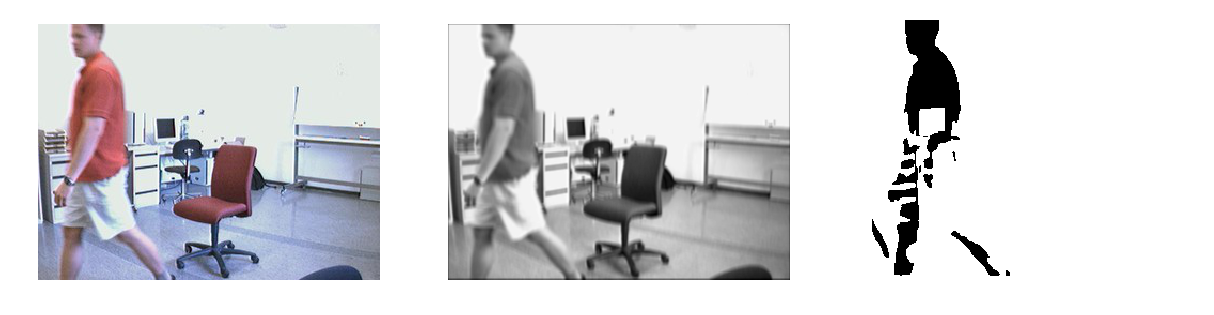
\includegraphics[width=0.46\textwidth]{margin.png}
\caption{Boundaries}
\label{bound}
\end{figure}



